% Figure 2: Lean4 Module Dependencies
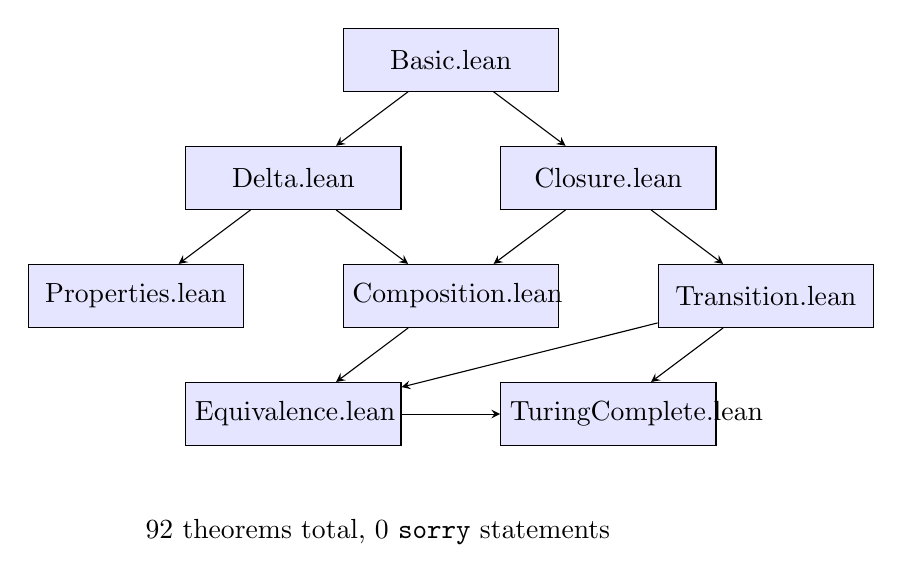
\begin{tikzpicture}[
    module/.style={rectangle, draw, fill=blue!10, text width=2.5cm, align=center, minimum height=0.8cm},
    arrow/.style={->, >=stealth}
]

% Top level
\node[module] (basic) at (4,6) {Basic.lean};

% Second level
\node[module] (delta) at (2,4.5) {Delta.lean};
\node[module] (closure) at (6,4.5) {Closure.lean};

% Third level
\node[module] (properties) at (0,3) {Properties.lean};
\node[module] (composition) at (4,3) {Composition.lean};
\node[module] (transition) at (8,3) {Transition.lean};

% Fourth level
\node[module] (equivalence) at (2,1.5) {Equivalence.lean};
\node[module] (turing) at (6,1.5) {TuringComplete.lean};

% Dependencies (arrows point from dependency to dependent)
\draw[arrow] (basic) -- (delta);
\draw[arrow] (basic) -- (closure);
\draw[arrow] (delta) -- (properties);
\draw[arrow] (delta) -- (composition);
\draw[arrow] (closure) -- (composition);
\draw[arrow] (closure) -- (transition);
\draw[arrow] (composition) -- (equivalence);
\draw[arrow] (transition) -- (equivalence);
\draw[arrow] (equivalence) -- (turing);
\draw[arrow] (transition) -- (turing);

% Legend
\node[anchor=west] at (0,0) {92 theorems total, 0 \texttt{sorry} statements};

\end{tikzpicture}
